\subsubsection{High Frequency vs Low Frequency pulses}\label{sssec:high_low_freq}
The pulse frequency is limited by the roundtrip time  of the transmitted photons. The roundtrip time can be calculated using \cref{eq:roundtrip}

\begin{align}\label{eq:roundtrip}
t_{round} = \frac{2r}{c}
\end{align}
where $c\approx 3\cdot10^8$ is the speed of light, and $r$ the altitude of the sensor. The maximum pulse frequency can then be calculated using \cref{eq:pulse_f}

\begin{align}\label{eq:pulse_f}
f_{pulse} = \frac{1}{t_{round}} = \frac{c}{2r}
\end{align}

The maximum altitude are different for the Altimetry and Hazard Detection mode. The maximum pulse frequency of both modes is shown in \cref{tab:pulse_frequency}.

\begin{table}[H]
\centering
\caption{Pulse frequency for both modes}
\label{tab:pulse_frequency}
\begin{tabular}{|l|ll|}
\hline
\textbf{Pulse Frequency}      &      Altimetry & Hazard Detection    \\ \hline
Maximum altitude  &  $8\,km$ & $500\, m$\\ 
Roundtrip time      &  $53.3\,\mu s$ & $3.33\,\mu s$ \\
Pulse frequency     & $18.75\,kHz$    & $300\,kHz$  \\ \hline
\end{tabular}
\end{table}


In order to increase the frequency, it is intersting to see what happens if the frequency is increased. The TDC measures the time between the last outgoing pulse and the incomming pulse. This means that the performed measurement $t_{TDC}$ can be calculated using \cref{eq:t_TDC_ToF}.

\begin{align}\label{eq:t_TDC_ToF}
	t_{TDC} &=ToF \mod T_{pulse}\\	
	ToF &= t_{TDC}+k\cdot T_{pulse} & k \in \mathbb{N}\label{eq:ToF_t_TDC}
\end{align}

 where $t_{TDC}$ is the measurement of the TDC, $ToF$ the time of flight, and $T_{pulse}$ the time period of the laser pulses. The returned answer is related to $ToF$ as shown in \cref{eq:ToF_t_TDC}. The precision of the measurement is maintained,  but on a larger scale the information is lost. \\
 \\
To solve this problem one can make measurements in two different frequencies. The idea is also applied in TDCs (Name of technique?), where two ring oscillators with different frequencies are used to amplify the range of the TDC. A similar idea can be applied here, but instead of using two oscillators, the time is devided in half, and in the first half the laser sends pulses in frequency $f_1$, and in the second half pulses with frequncy $f_2$. These two different measurements can first be used to determine the large scale ToF, and then the measurements can be combined to get a high accuracy to accompany that.\\
\\
As a proof of concept. This idea is applied to the Altimetry Mode. It is assumed that a difference of $5\,ns$ between $\lambda_1$ and $\lambda_2$ is sufficient. Now using a maximum $ToF$ one can calculate that optimal two frequencies, such that $f1_>f_2$ and $f_2$ as high as possible. 

\begin{align}
 	\frac{50\mu}{5n} &= 10660\\ 
 	\sqrt{\frac{50\mu}{5n}} &\approx 103
 \end{align} 
 Now two coprime numbers in $\mathbb{N}$ around 103 are 103 and 104. The resulting frequencies are
 \begin{align}
 	T_1 &= 103\cdot5n = 515n\\
 	T_2 &= 104\cdot5n = 520n\\
 	f_1 &= \frac{1}{T_1} = 1.9417\,MHz\\
 	f_2 &= \frac{1}{T_1} = 1.9231\,MHz\\
 \end{align}
The pulse frequency increases by a factor 100. A matlab plot of the resulting system is shown in \cref{fig:frequency_hopping}, where the measurement values of the TDC are plotted against the $ToF$.


\begin{figure}[h]
    \centering
    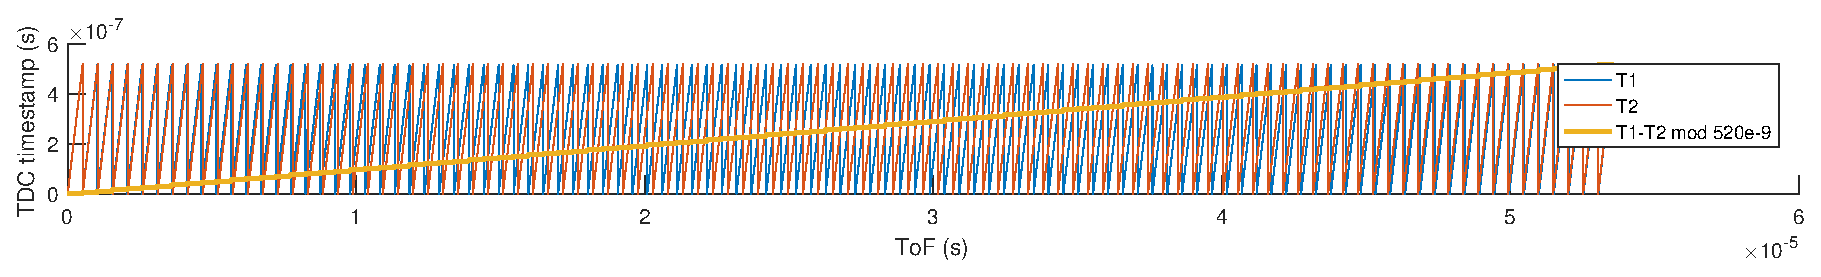
\includegraphics[width=\textwidth]{fig/frequency_hopping.eps}
    \caption{Matlab plot of TDC measurements vs ToF}
    \label{fig:frequency_hopping}
\end{figure}

The $ToF$ can be calculated using \cref{eq:ToF}.

\begin{align}
	t_{1-2} &= (t_1-t_2)\mod T_2\\
	ToF &= \frac{t_{1-2}}{T_2-T_1}T_1+\frac{t_1+t_2-t_{1-2}}{2}\label{eq:ToF}
\end{align}
where $t_1$ and $t_2$ are the timestamp measurements for $f_1$ and $f_2$ respectively. $t_{1-2}$ is the modulus of the time difference between $t_1$ and $t_2$.
